
\subsection{CW-NIR laser effect on spike waveform}
In this paper we performed experimental triplets of control, sustained CW-NIR laser stimulation and recovery recordings (for details see Sec. \ref{sect:sustained-protocol}). This protocol provided a reference for the characterization of the laser effect. The data analyzed in this section corresponds to the spontaneous activity of neurons from the right parietal ganglion (RPG) of \textit{Lymnaea stagnalis}, under no stimulation other than the laser illumination when specified.

Left panels in Fig. \ref{fig:continuous_results_panel}A and B illustrate the stereotyped waveform of the action potential from two experiments in two distinct neuron types present in the RPG with symmetrical and shoulder spike shapes, respectively. Note that the two neuron types differ not only in spike waveform but also in duration. In the example shown in Fig. \ref{fig:continuous_results_panel}A, the duration of the spike was $\sim$20 ms whereas the one shown in Fig. \ref{fig:continuous_results_panel}B was $\sim$40-50 ms. To characterize the sustained CW-NIR laser stimulation in terms of change and recovery, the three stages of the protocol --control, laser and recovery-- are represented in all panels. The superimposition of the spike waveforms ($\sim$40 and 110 spikes for each trial, panels A and B, respectively) for the same recording are aligned in the $x$ axis by the spike peak and in the $y$ axis by the voltage amplitude of the first point of the waveform, together with the trial mean spike represented with a wider line. Note how the control and recovery traces overlap for both neuron types, illustrating the resumption of the spike dynamics shortly after the laser stimulation ceases (see aligned spikes in Fig. \ref{fig:continuous_results_panel} A and B).

Figures \ref{fig:continuous_results_panel}A and B illustrate that the variability was very small in amplitude, duration and in depolarization or repolarization slopes between the spikes within the same trial in both neuron types. However, during CW-NIR laser stimulation, the change in action potential waveform shape was notable with respect to the control and the recovery. This change was most clear in the spike duration, which was the result of changes in both depolarization and repolarization slopes. 

\begin{figure}[htb!]
	\centering
	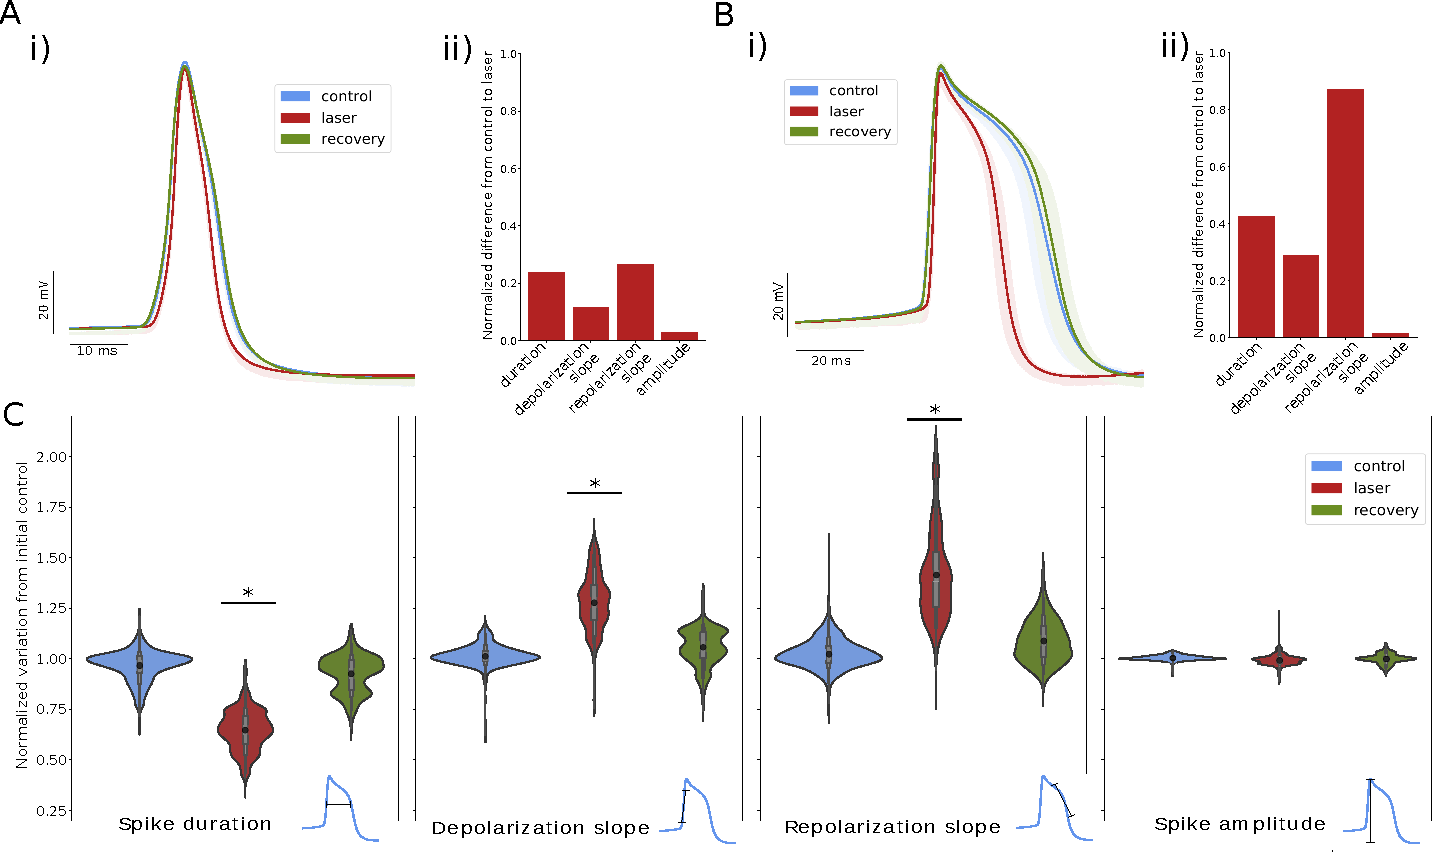
\includegraphics[width=\textwidth]{img/laser/Figure2.pdf}
	\caption{Effect of sustained CW-NIR laser stimulation on the spike waveform for two distinct neuron types. For all panels: control, laser and recovery are color coded in blue, red and green, respectively. Panel A. Characterization of no shoulder shape type neuron. Panel B. Characterization of shoulder shape type neuron. Ai) and Bi) Superimposition of spike waveforms in a single trial recording corresponding to a symmetrical and shoulder spike neuron, respectively. The spikes were aligned to the peak for the $x$ axis and to the onset for the $y$ axis, the mean is depicted in darker colors. Aii) and Bii) barcharts quantify the change using the difference from laser to control normalized by the mean control value for metrics: duration, depolarization and repolarization slopes, and amplitude. Panel C, violin plots representing the variation of the experiments with respect to the control ($N=23$) for shoulder and symmetrical types together. For each metric of the waveform, the control, laser and recovery recordings are normalized to the first control. From left to right: duration, depolarization slope, repolarization slope and amplitude. Asterisks over the violins indicate that the metric change was highly significant (Bonferroni correction, ($\rho<0.01/4$), see Statistical Analysis Sec. \ref{sect:statistical_analysis} in Materials and Methods).}
	\label{fig:continuous_results_panel}
\end{figure}

The right panels ii) in Fig. \ref{fig:continuous_results_panel}A and B, show barcharts that quantify the change in terms of spike duration, amplitude, depolarization slope and repolarization slope. These metrics were used to characterize the action potential waveform and its possible change during the laser illumination (see also Fig. \ref{fig:methods_general}B and Sec. \ref{sect:metrics}). Each one of these metrics is represented on the right panels as the absolute value of the difference of the laser stimulation to the control recording normalized by the mean control value (see Sec. \ref{sect:statistical_analysis}). For both neuron types there was a change in duration and in the slopes, with the largest change being in the repolarization slope (around 26\% for the symmetrical spike type neuron and 86\% for the shoulder type). The alignment illustrated in the left panels shows that the change in amplitude was minimal in comparison to the rest of the metrics. Although both neuron types showed an effect of the sustained CW-NIR laser stimulation in the action potential waveform, the change in the shoulder neuron type was larger for duration and slopes. This may be due to specific channels that generate the shoulder shape of the spike, which may allow for a wider range of change in the spike dynamics, especially in terms of the repolarization slope. 


Panel C in Fig. \ref{fig:continuous_results_panel} displays the results of multiple experiments following the same protocol described above, represented in violin plots as the normalization of each experiment with respect to the mean of the first control of the respective metric for each spike detected during control, laser and recovery. To avoid possible bias from the natural evolution of the intracellular recordings, in this figure we only included experiments where the activity was recovered within 10\% change in firing rate with respect to the control. For each trial, only stereotyped waveforms were considered and large deviations (in the form of $z_{score} < -0.1$ in the normalized duration) were filtered out. The variability characterized in the control violins represents the variation within controls, which was also the most homogeneous in terms of density distribution. This is represented for each one of the selected spike waveform characterization metrics as in panels A and B --duration, depolarization slope, repolarization slope and spike amplitude (see Fig. \ref{fig:methods_general}B).

The results shown in Fig. \ref{fig:continuous_results_panel}, panel C are consistent with the described change in the illustrative individual experiments shown in panels A and B in the same figure. On the one hand, the activity recovered its initial characteristics after the CW-NIR laser stimulation ceased for every metric, i.e., the recovery (green violin) returned to the same level as the control (blue violin). The differences in these distributions are mainly caused by the natural variability in the biological system. Also, as all values are normalized to the mean of the first control, it can be expected that the distributions may diverge more in laser and recovery violins than in control violins. A separate analysis for the two neuron types is available in Fig. \ref{fig:continuous panel s1}

\begin{figure}
	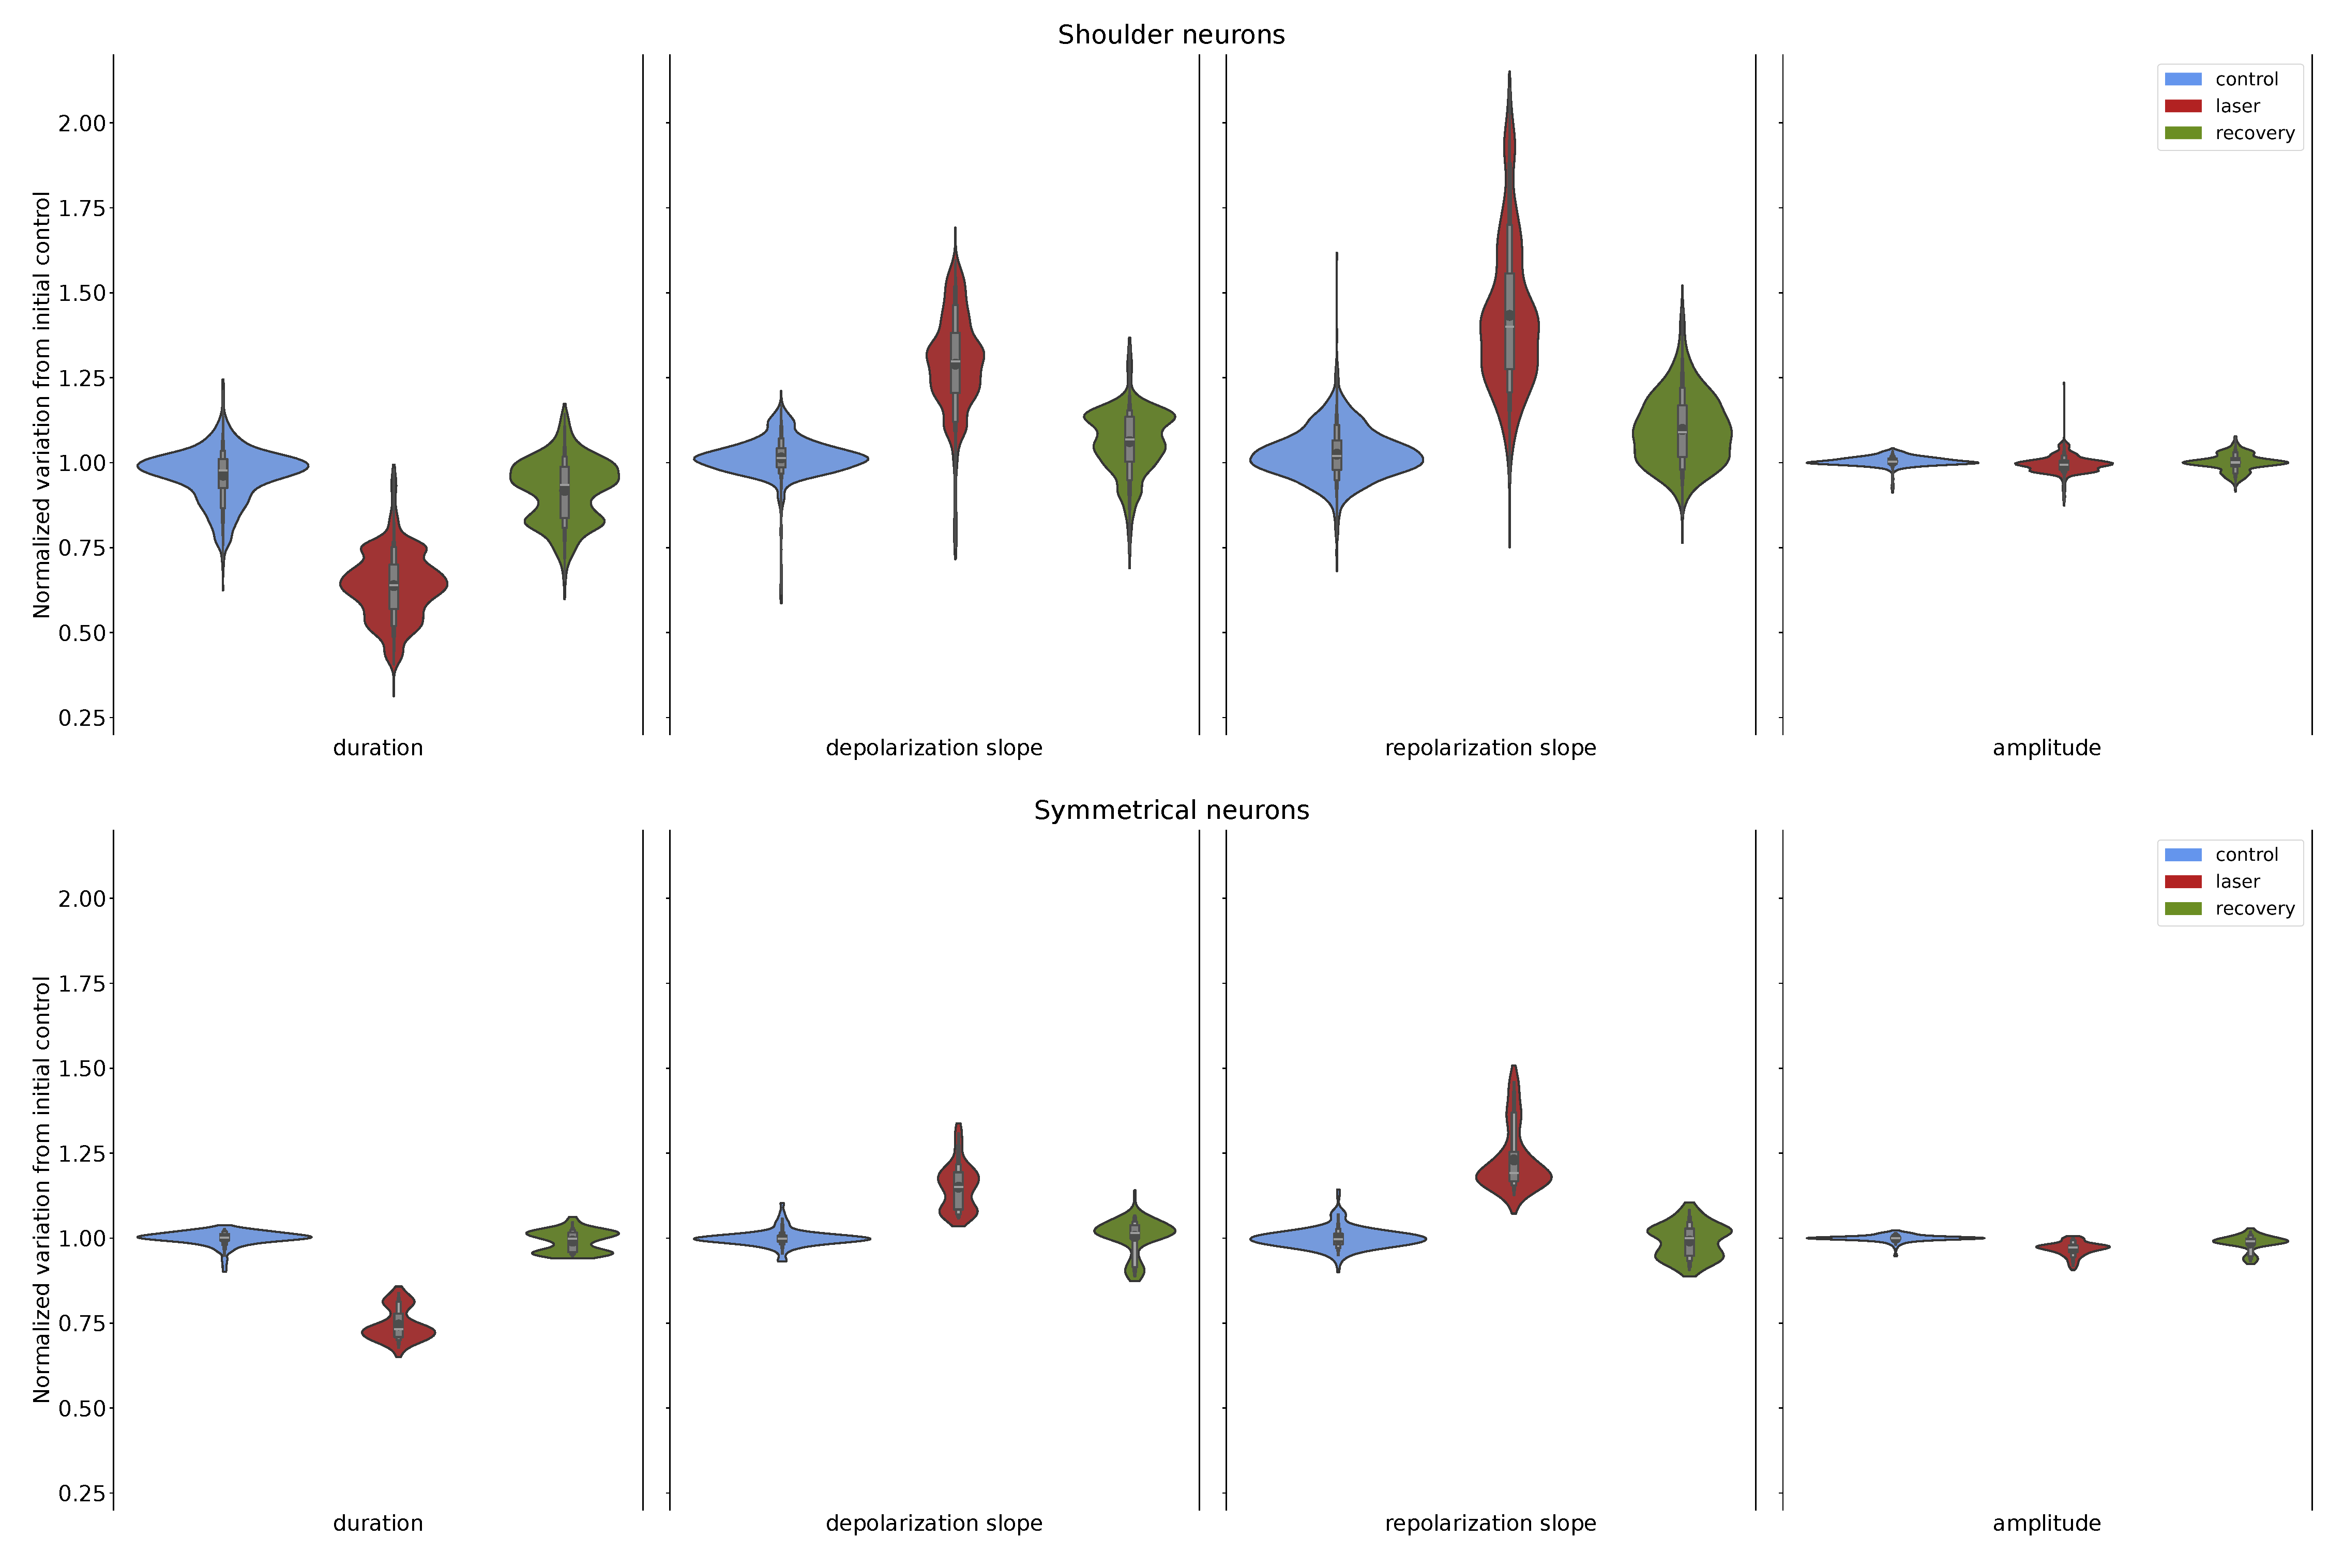
\includegraphics[width=\textwidth]{img/laser/FigureS1.eps}
	\caption{Segregation of data into shoulder and symmetrical neural types. Violin plots for the four metrics -duration, depolarization slope, repolarization slope and amplitude- grouped by control, laser and recovery trials. Spikes metrics are normalized to the first control, as in Fig. \ref{fig:continous_results_panel} panel C}
	\label{fig:continous panel s1}
\end{figure}

Regarding the change during the laser stimulation, for every waveform metric except amplitude, we can see in Fig. \ref{fig:continuous_results_panel}C how the overlapping of the distributions is minimal. The distribution for the duration was the most homogeneous, whereas the variation for depolarization and repolarization slopes had different density distributions, being the repolarization slope the one presenting a larger change in most cases. This can be explained by the variety of neurons in the collected data, the change in the slopes differed from one type of neuron to another. Thus, the distribution of variability was different. Some laser stimulation recordings presented a milder change than others. The slight change along neurons of the same type was likely due to the physical restrictions of the setup in each experiment: the angle of the laser, the laser focusing, the maximum power used and the overlaying tissue. Overall, considering these factors, we can see that stimulating with the sustained CW-NIR laser resulted in a significant change of the spike waveform. In the case of the amplitude, the change was very small. 

We performed statistical tests on these data and confirmed that the changes in duration, depolarization and repolarization slopes were highly significant ($\rho < 0.01 /4$) when comparing control and laser samples. The amplitude change was not highly significant, and so were not the changes in any metric comparing control and recovery samples (see Statistical Analysis Sec. \ref{sect:statistical_analysis}).

This combination of changes points out to different biophysical candidates that might be involved in the modulation for the global change in both slopes or specific channels involved in the CW-NIR laser effect, since the deporalization and repolarization slopes were affected differently, while the amplitude did not change, and for distinct neuron types the characterized metrics had different variations (i.e., the repolarization slope in the shoulder shape neuron type was reduced to a greater extent than in the symmetrical type). In section \ref{sect:models} we assess these possible candidates using a computational model. 

\subsection{CW-NIR laser effect on spiking rate}
During the identification of the biophysical effect at different phases of the action potential dynamics on single neurons, we identified a robust acceleration of the action potential (a shorter duration of the spike waveform). This could also point to an acceleration of the tonic activity of the neurons. Pulsed NIR laser stimulation has been proven effective as a stimulation technique, mainly eliciting action potentials (APs) in silent neurons at specific combinations of pulse duration and intensity \parencite{wells_application_2005, shapiro_infrared_2012, izzo_optical_2007, cayce_infrared_2014}. Thus, we also assessed the effect during sustained CW-NIR infrared laser stimulation on the spiking frequency in long stimulation recordings (1-3 min). 

To avoid possible bias originated from intrinsic properties of the neuron and the circuit in which it was integrated, we only considered recordings where the neurons effectively recovered their control activity rate after the stimulation (i.e., absolute recovery change within 10\% from the initial control). The activity frequency was characterized by the absolute firing rate (AFR) for control, laser and recovery, and by a histogram of Inter Spike Intervals (ISIs), i.e., the time interval from peak to peak.

\begin{figure}[hb!]
	\centering
	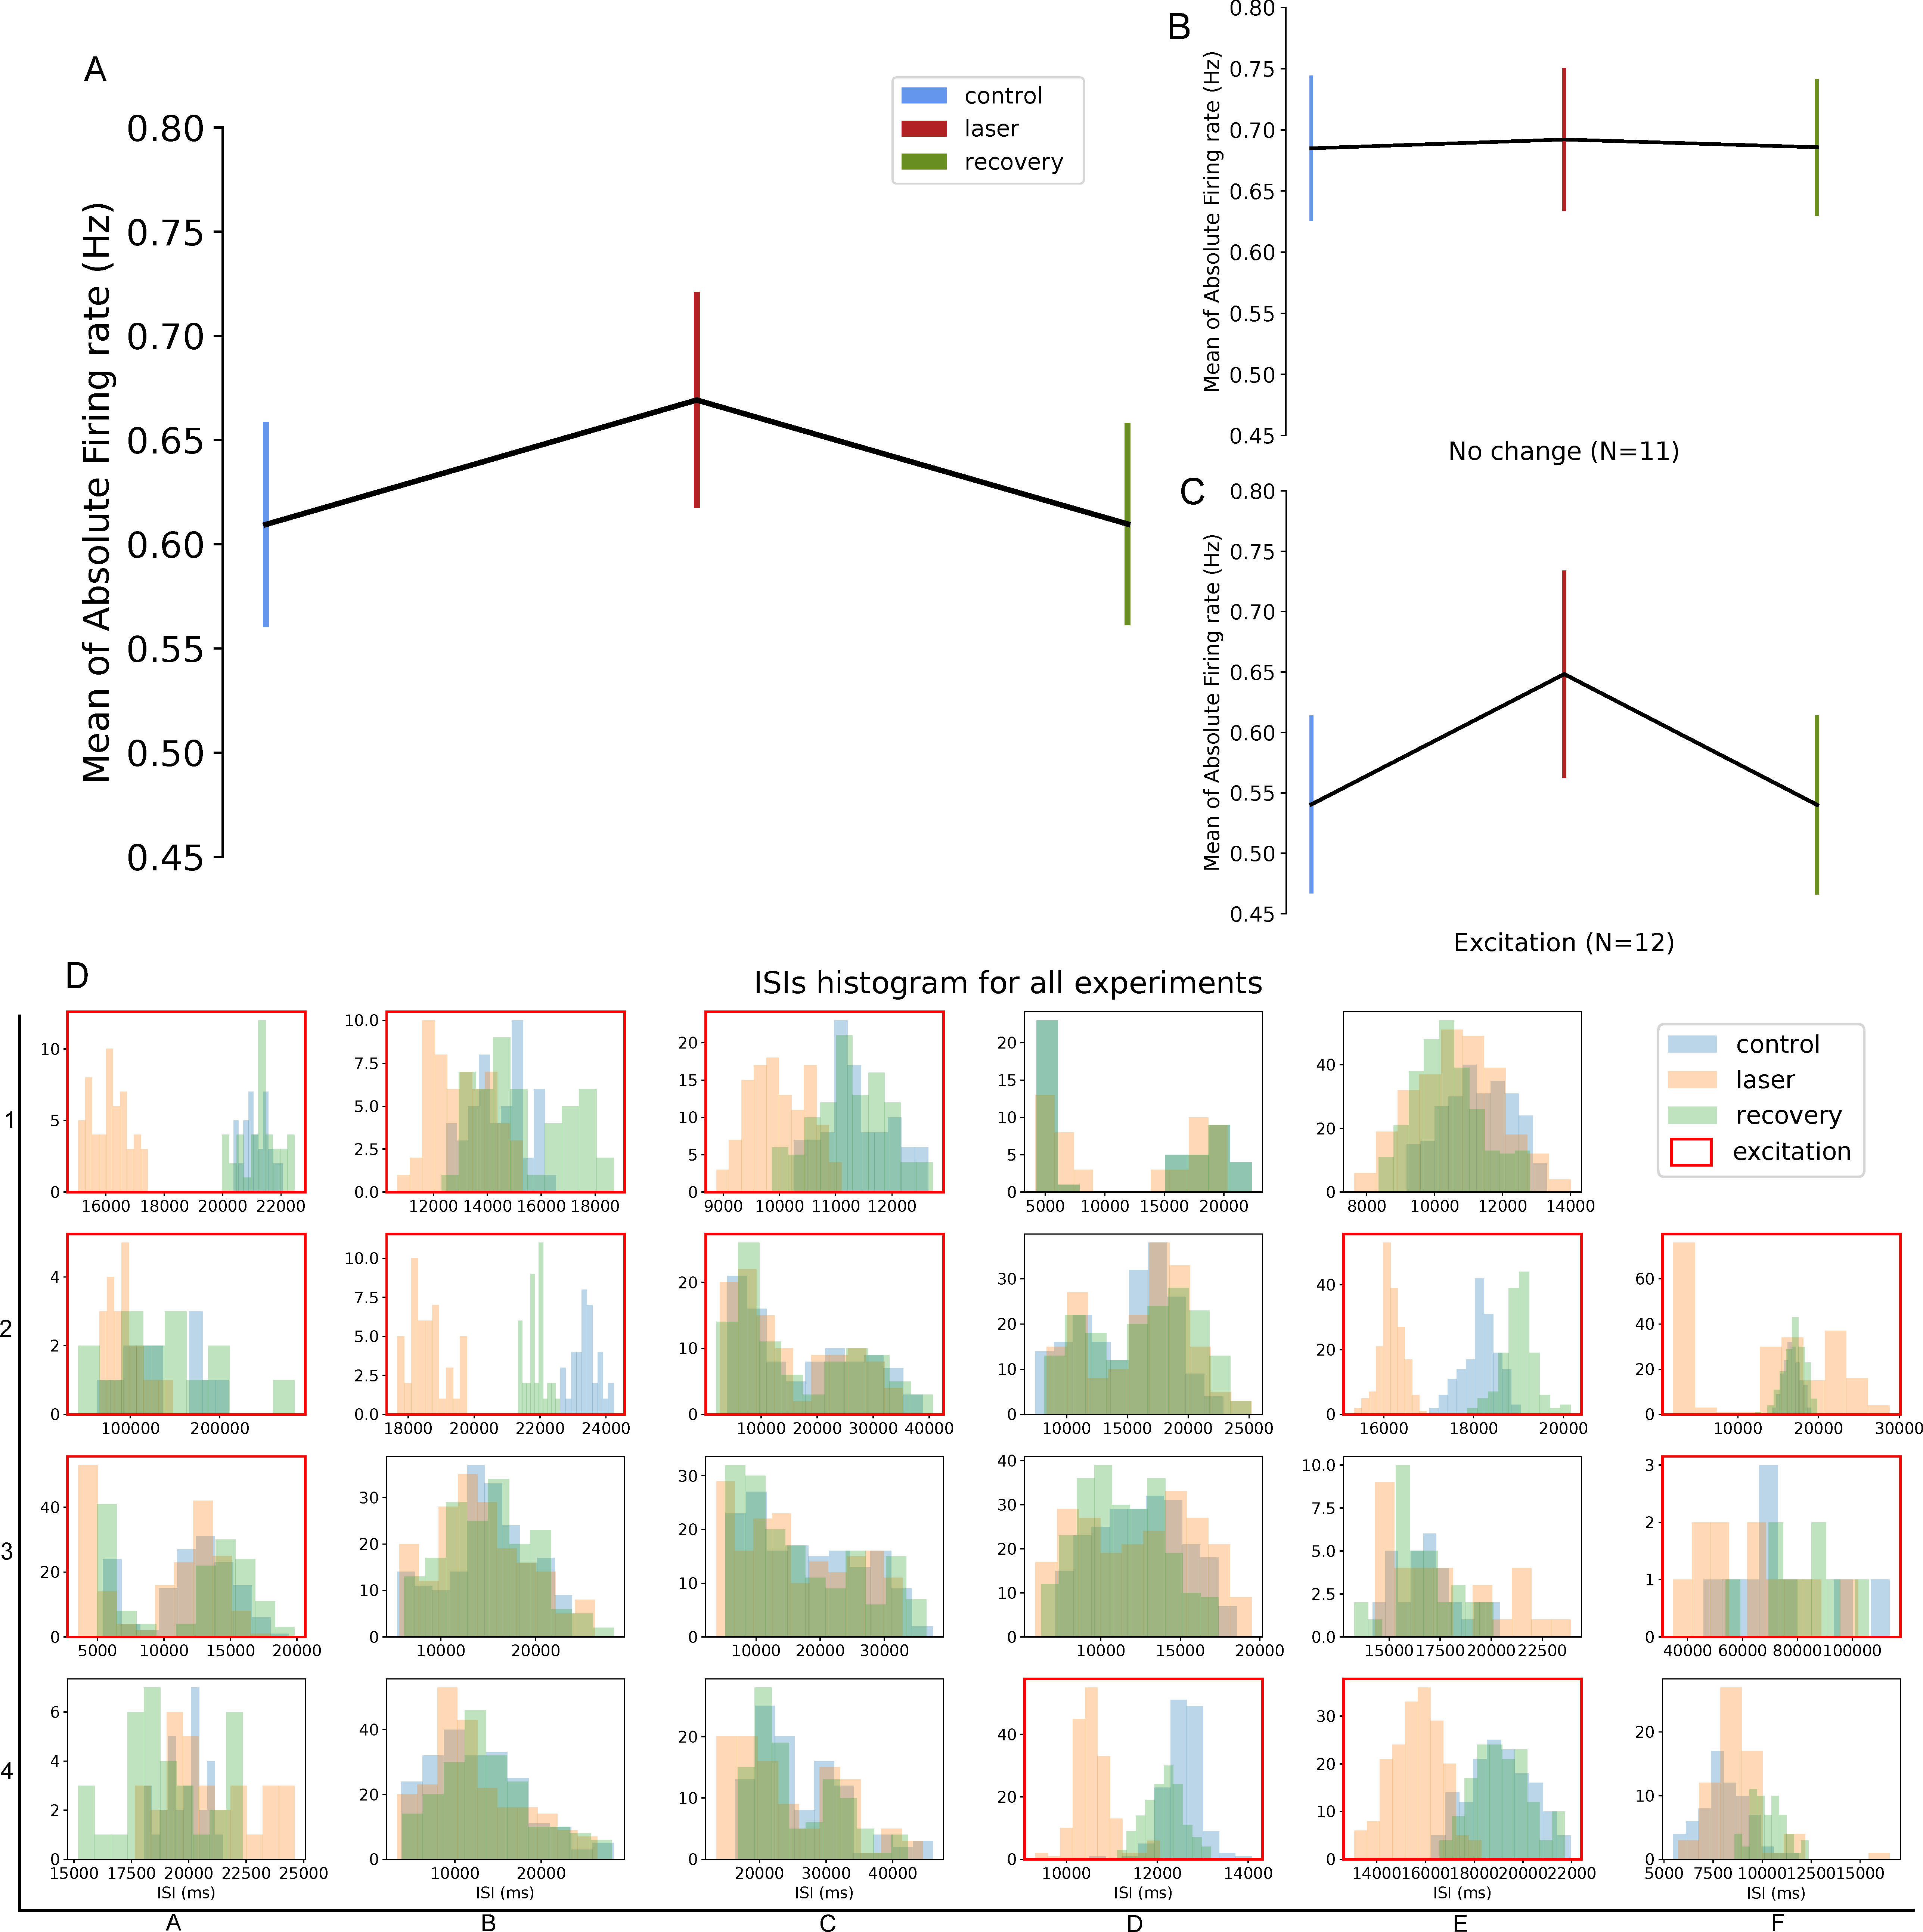
\includegraphics[width=\textwidth]{img/laser/Figure3.pdf}
	\caption{Firing rate and interspike interval (ISIs) analysis for the CW-NIR laser stimulation. A. Absolute firing rate in all experiments (N=23). B. Absolute firing rate for cases from the experiments in A with no change during laser illumination (N=11); C. Absolute firing rate for experiments from A showing an increase in the firing rate (N=12); D. ISI histograms for control, laser and recovery for each experiment. Cases showing increased excitation in their firing rate (sample in panel C) when illuminated by the CW-NIR laser are highlighted in a red square.}
	\label{fig:frequency FR}
\end{figure}

In Fig. \ref{fig:frequency FR}, the mean firing rates for control, laser and recovery are represented along with their standard error of the mean. Panel A depicts the general change in frequency for the neurons, showing the neural activity trend to excitation in the mean. In panels B and C, this set of triplets is divided into two groups depending on the difference between the laser and the control, classified as no change when the difference between control and laser was less than 10\% (panel B), and as excitation for the opposite case (panel C). There is no representation of inhibition in this panel, since there was not any experiment that fulfilled the criteria of a 10\% negative change during the laser stimulation with respect to the control. Note how cases where the activity increases are the most consistent ones (12 out of 23) and that even in the set classified as unchanged, the mean of the AFR during laser stimulation is larger than the controls. These results support an excitatory tendency during CW-NIR sustained stimulation.

The absolute firing rate hinders some characteristics of the neural activity, such as the refractory period or the presence of bursting activity, which might also influence the firing frequency study. Thus, Fig. \ref{fig:frequency FR}D displays the ISI histogram for each experiment showing again the triplets of control, laser and recovery, for each sample. Experiments showing excitation are highlighted in a red square. Note that for most cases classified as excitation, the ISIs tendency is to be reduced, which is observed in the laser histogram at the left of the control and the recovery. Note that there are some experiments where the laser ISI histogram seems to overlap with the controls and the recovery (see Fig. \ref{fig:frequency FR}D, panels [2,A] [3,A] and [2,C]) but still the mean AFR of the laser recording was 10\% higher than the control. In these situations, even though the activity was faster under stimulation, the time between spikes did not show a proportional change, which can be due to a modulation in the refractory period that compensated the spike acceleration. Under the laser modulation, we also found that some neurons would start firing in shorter ISIs, tuning the tonic spiking into pair spiking similar to small bursts, e.g. Fig. \ref{fig:frequency FR}D, panel [2,F].

Overall, our results in this subsection show a larger tendency to a frequency increase in response to the NIR illumination indicating that it is possible to achieve neuronal excitation under sustained CW-NIR laser stimulation. It is also important to highlight that inhibition was not found in any of these experiments with sustained CW-NIR laser stimulation during tonic firing activity. 


\subsection{Effect of CW-NIR stimulation in a minimal circuit}


\subsection{Effect of CW-NIR stimulation at different wavelengths}

\begin{figure}[hbt]
	\centering
	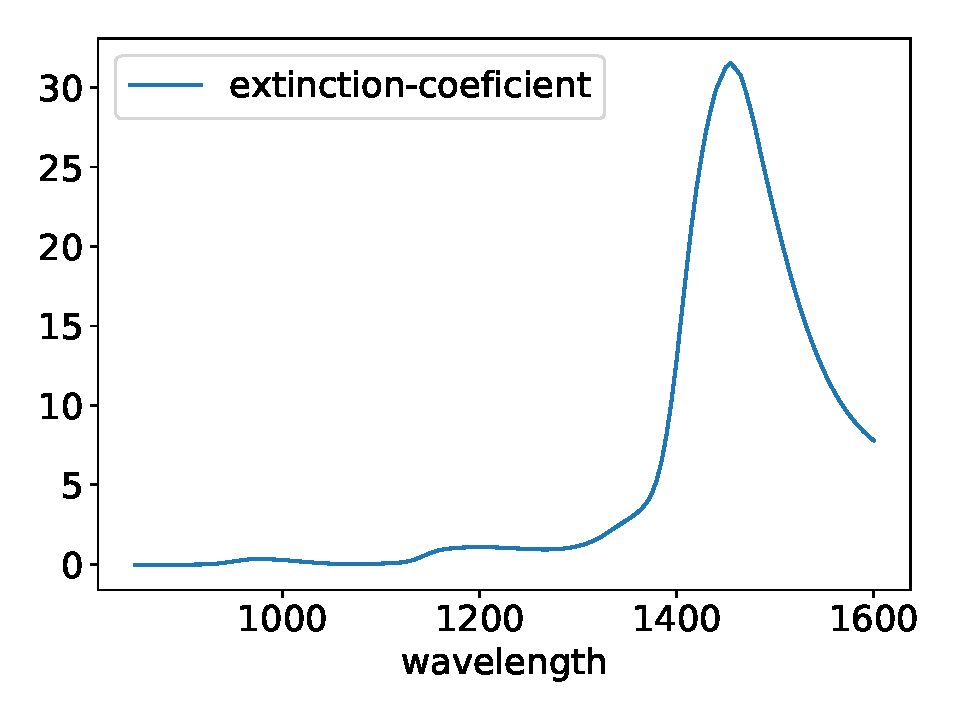
\includegraphics[width=0.9\textwidth]{img/laser/wavelength/water_absoption_wavelength.pdf}
\end{figure}

\begin{figure}[hbt]
	\centering
	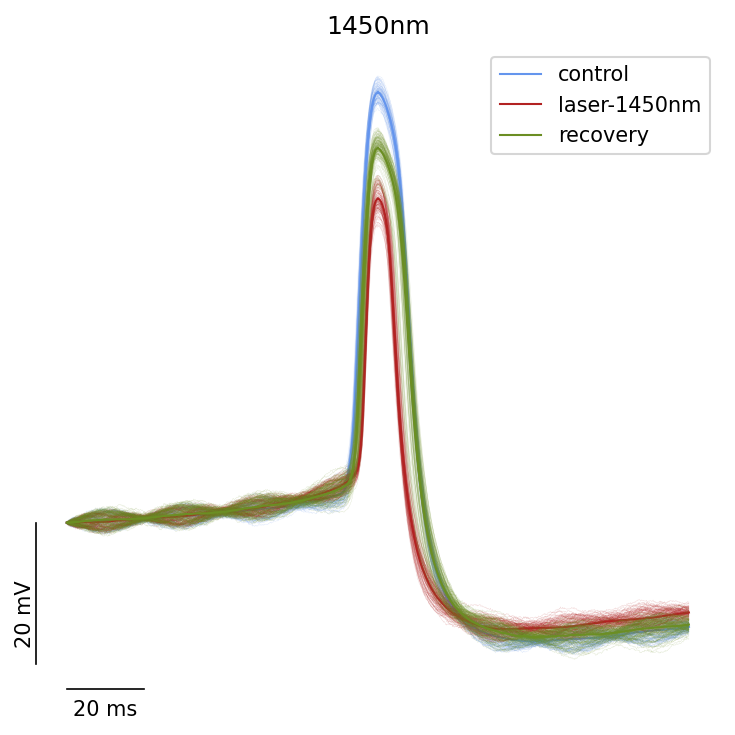
\includegraphics[width=0.2\textwidth]{img/laser/wavelength/1450nm.png}
	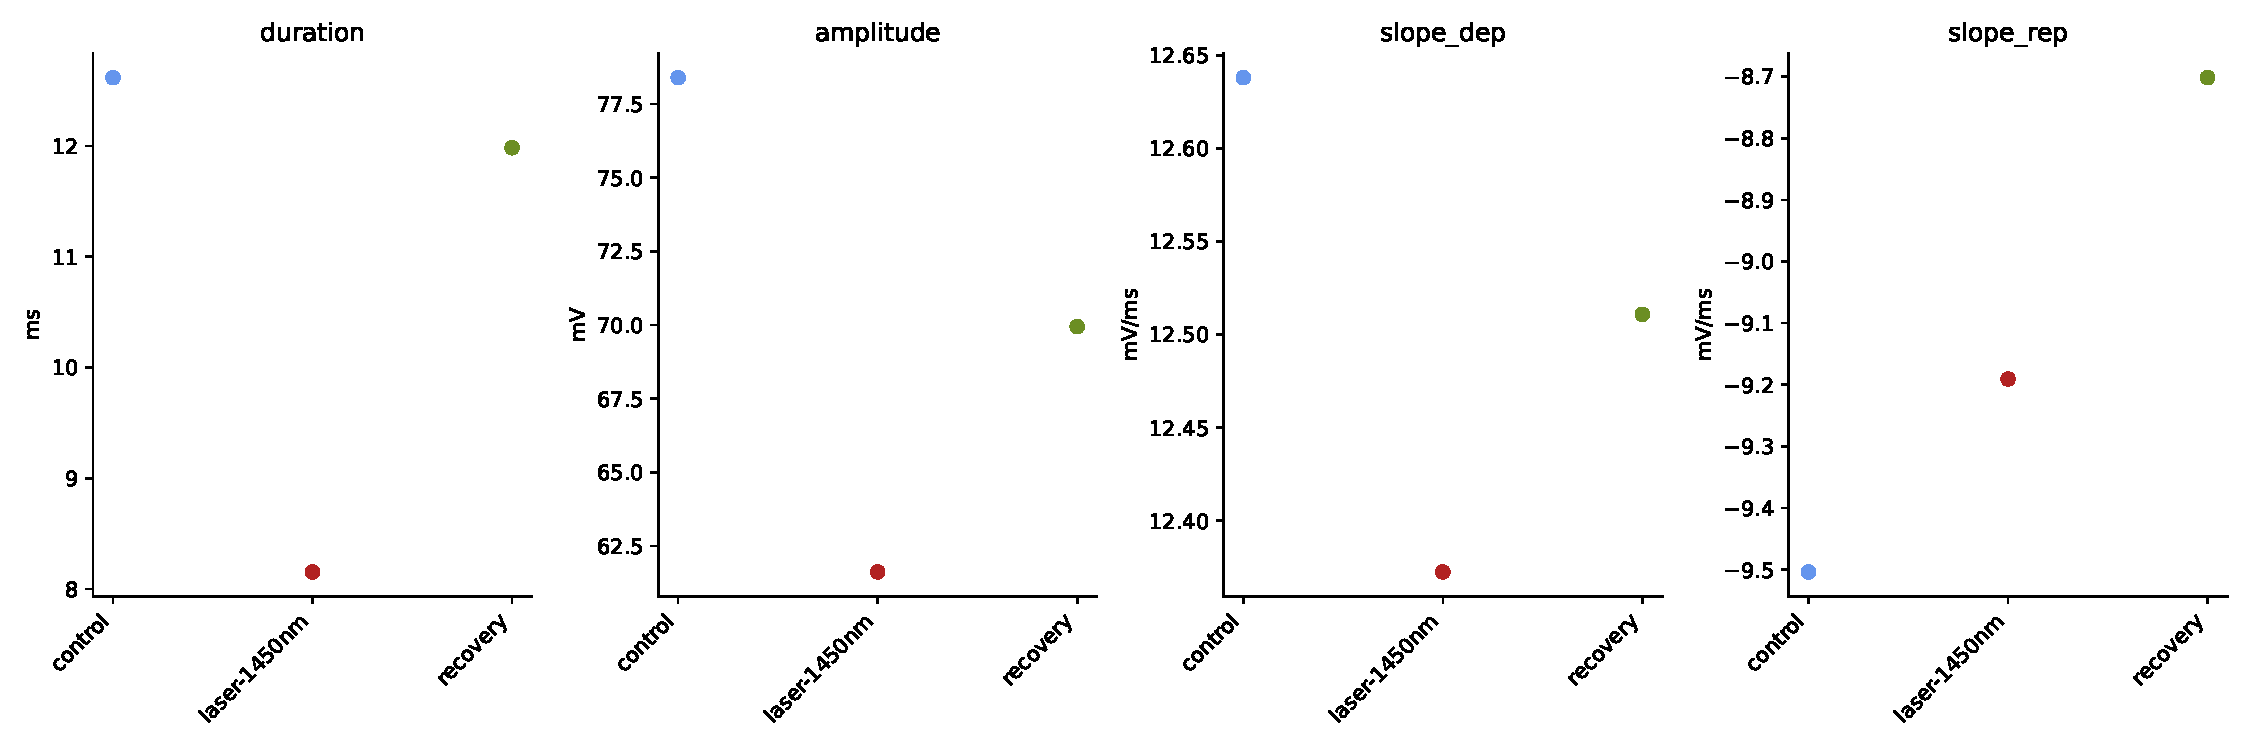
\includegraphics[width=0.6\textwidth]{img/laser/wavelength/1450nmmetrics.pdf}
\end{figure}


\begin{figure}[hbt]
	\centering
	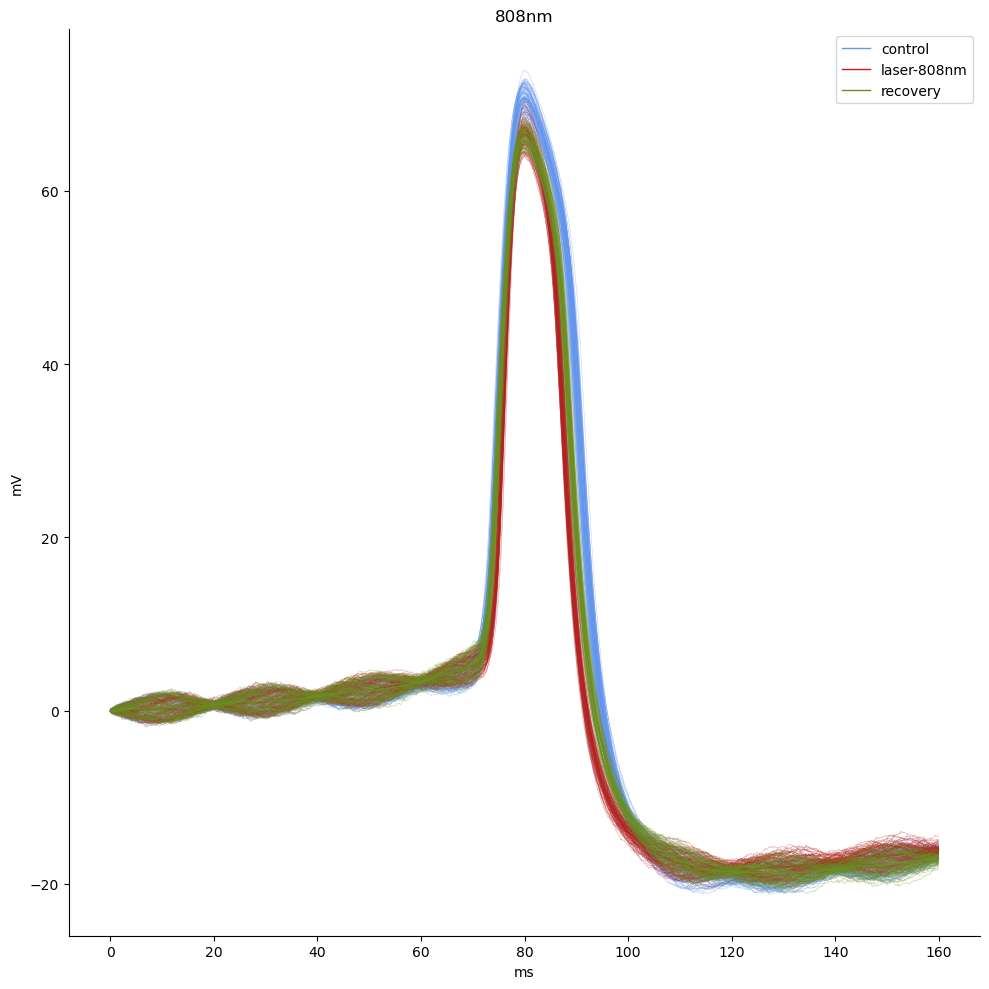
\includegraphics[width=0.2\textwidth]{img/laser/wavelength/808nm.png}
	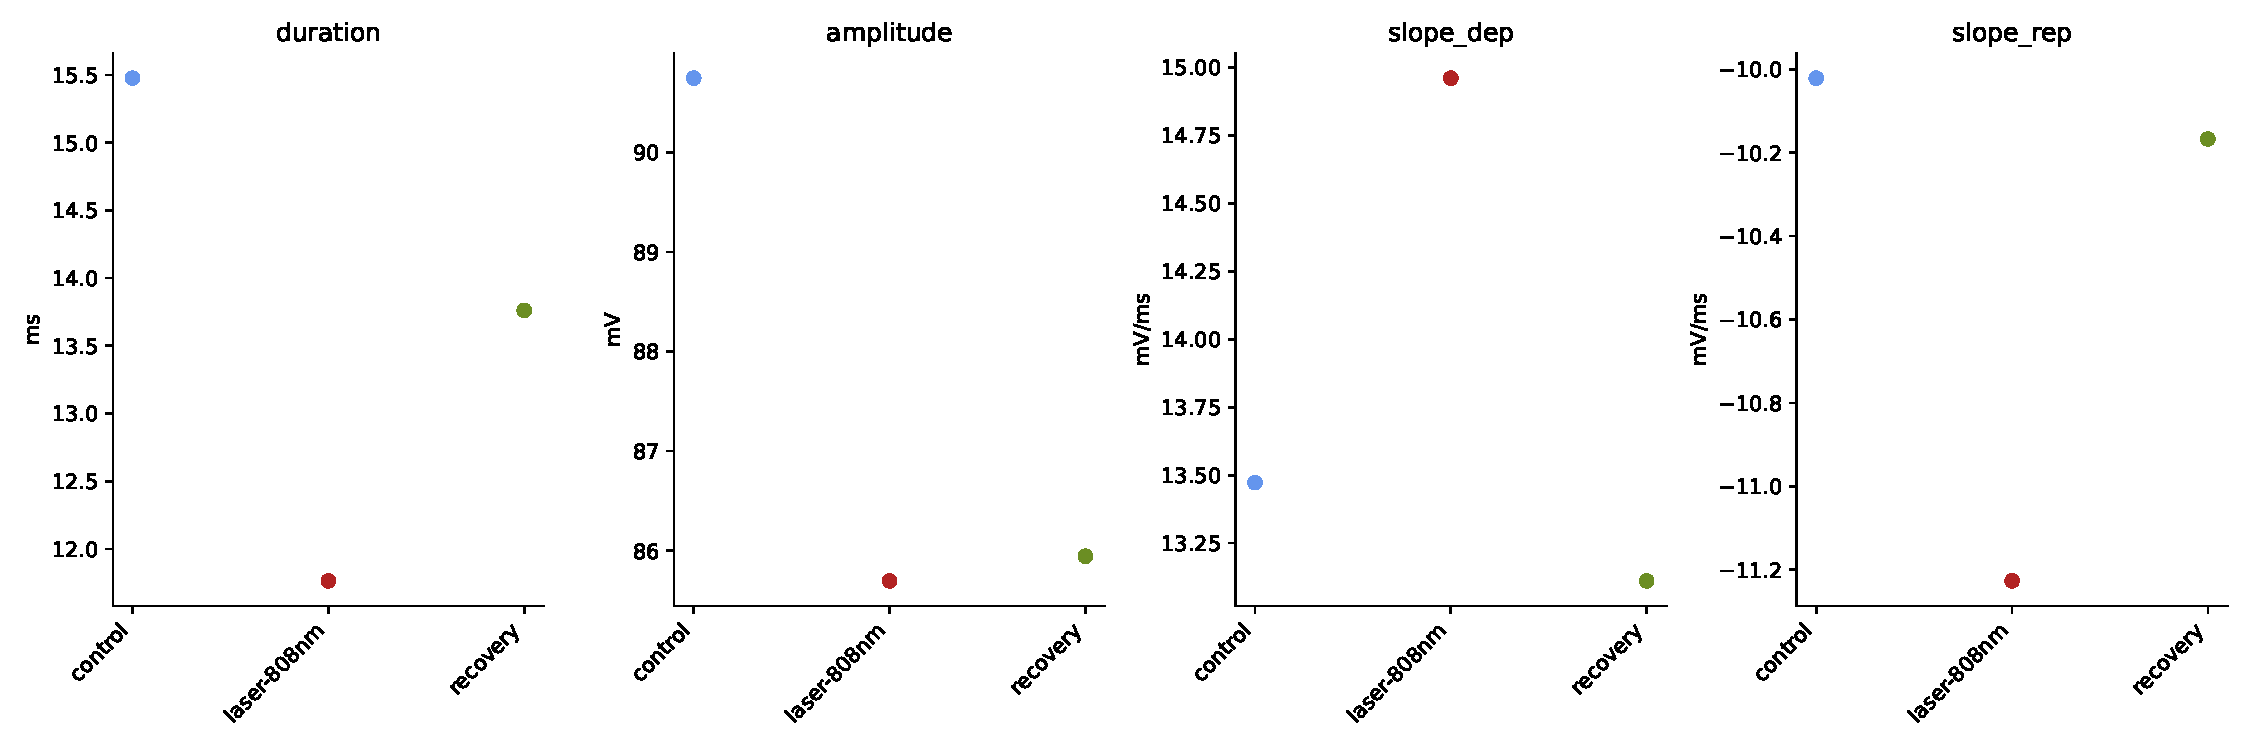
\includegraphics[width=0.6\textwidth]{img/laser/wavelength/808nmmetrics.pdf}
\end{figure}

\begin{figure}[hbt]
	\centering
	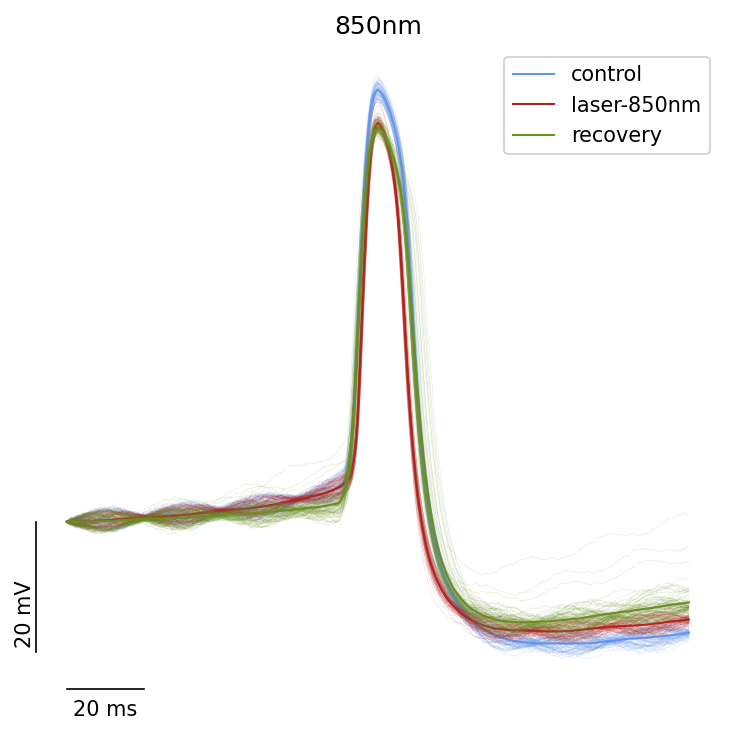
\includegraphics[width=0.2\textwidth]{img/laser/wavelength/850nm.png}
	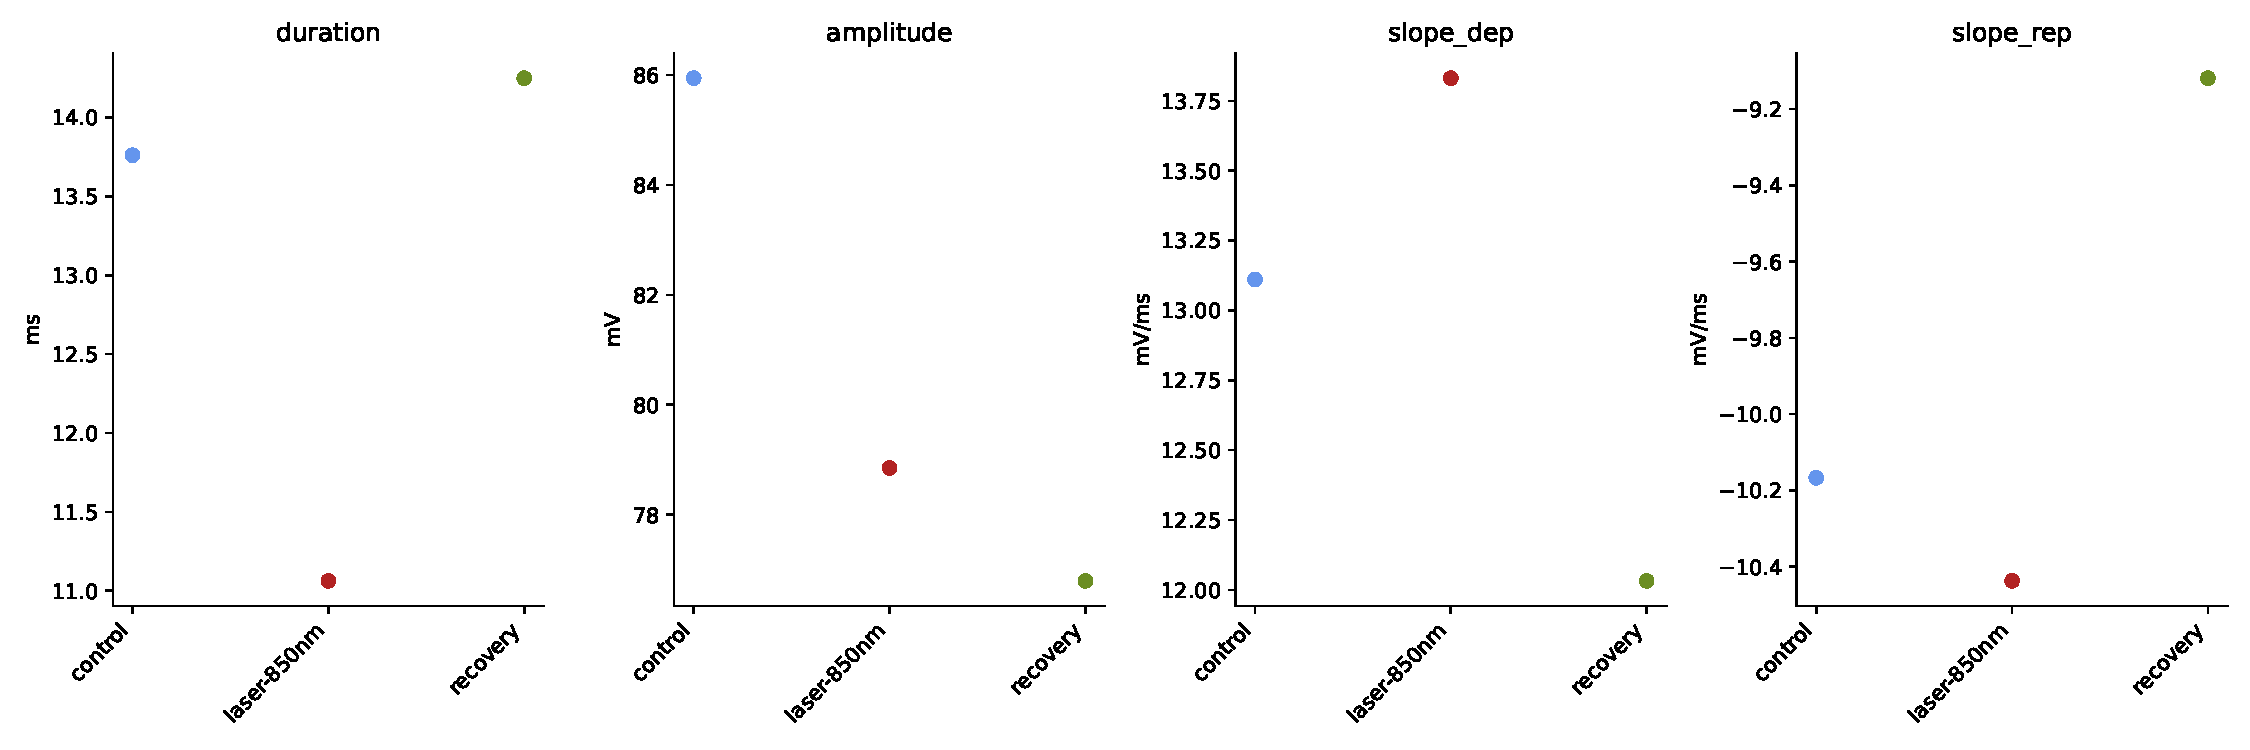
\includegraphics[width=0.6\textwidth]{img/laser/wavelength/850nmmetrics.pdf}
\end{figure}

\begin{figure}[hbt]
	\centering
	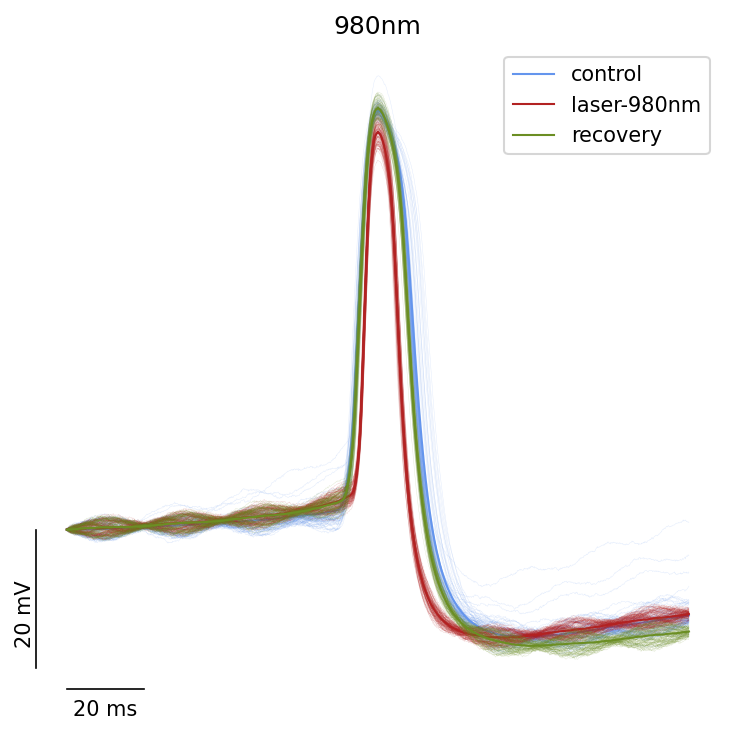
\includegraphics[width=0.4\textwidth]{img/laser/wavelength/980nm.png}
	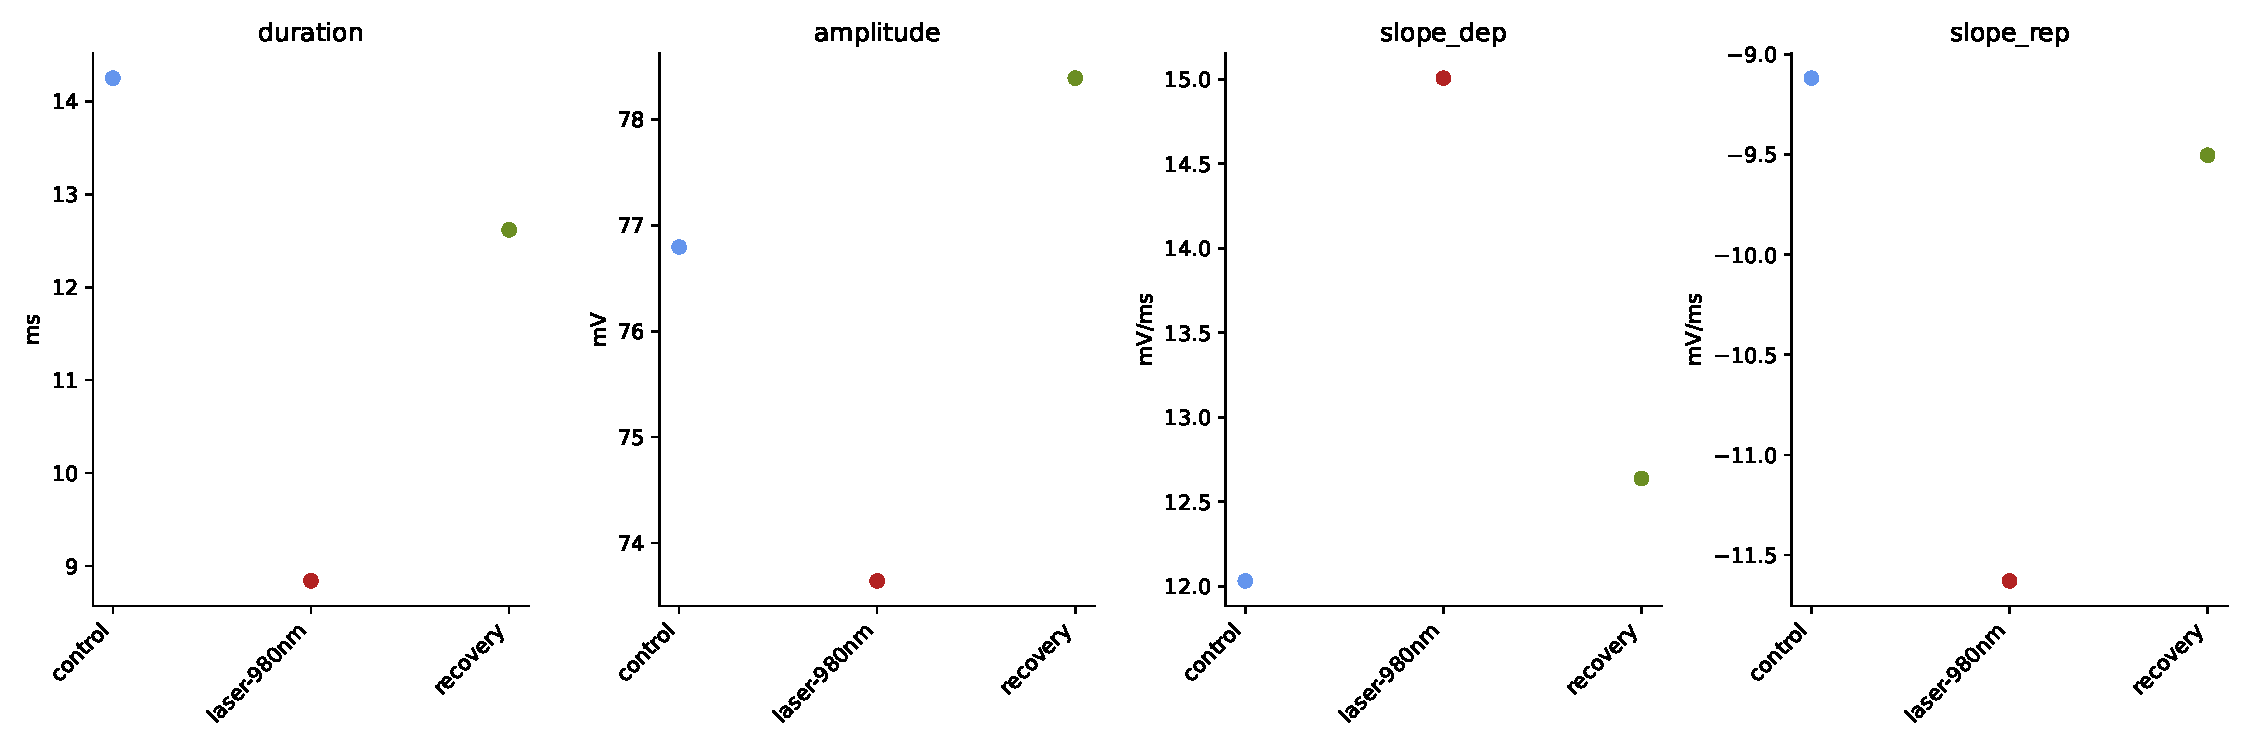
\includegraphics[width=0.3\textwidth]{img/laser/wavelength/980nmmetrics.pdf}
\end{figure}



\begin{figure}[hbt]
	\centering
	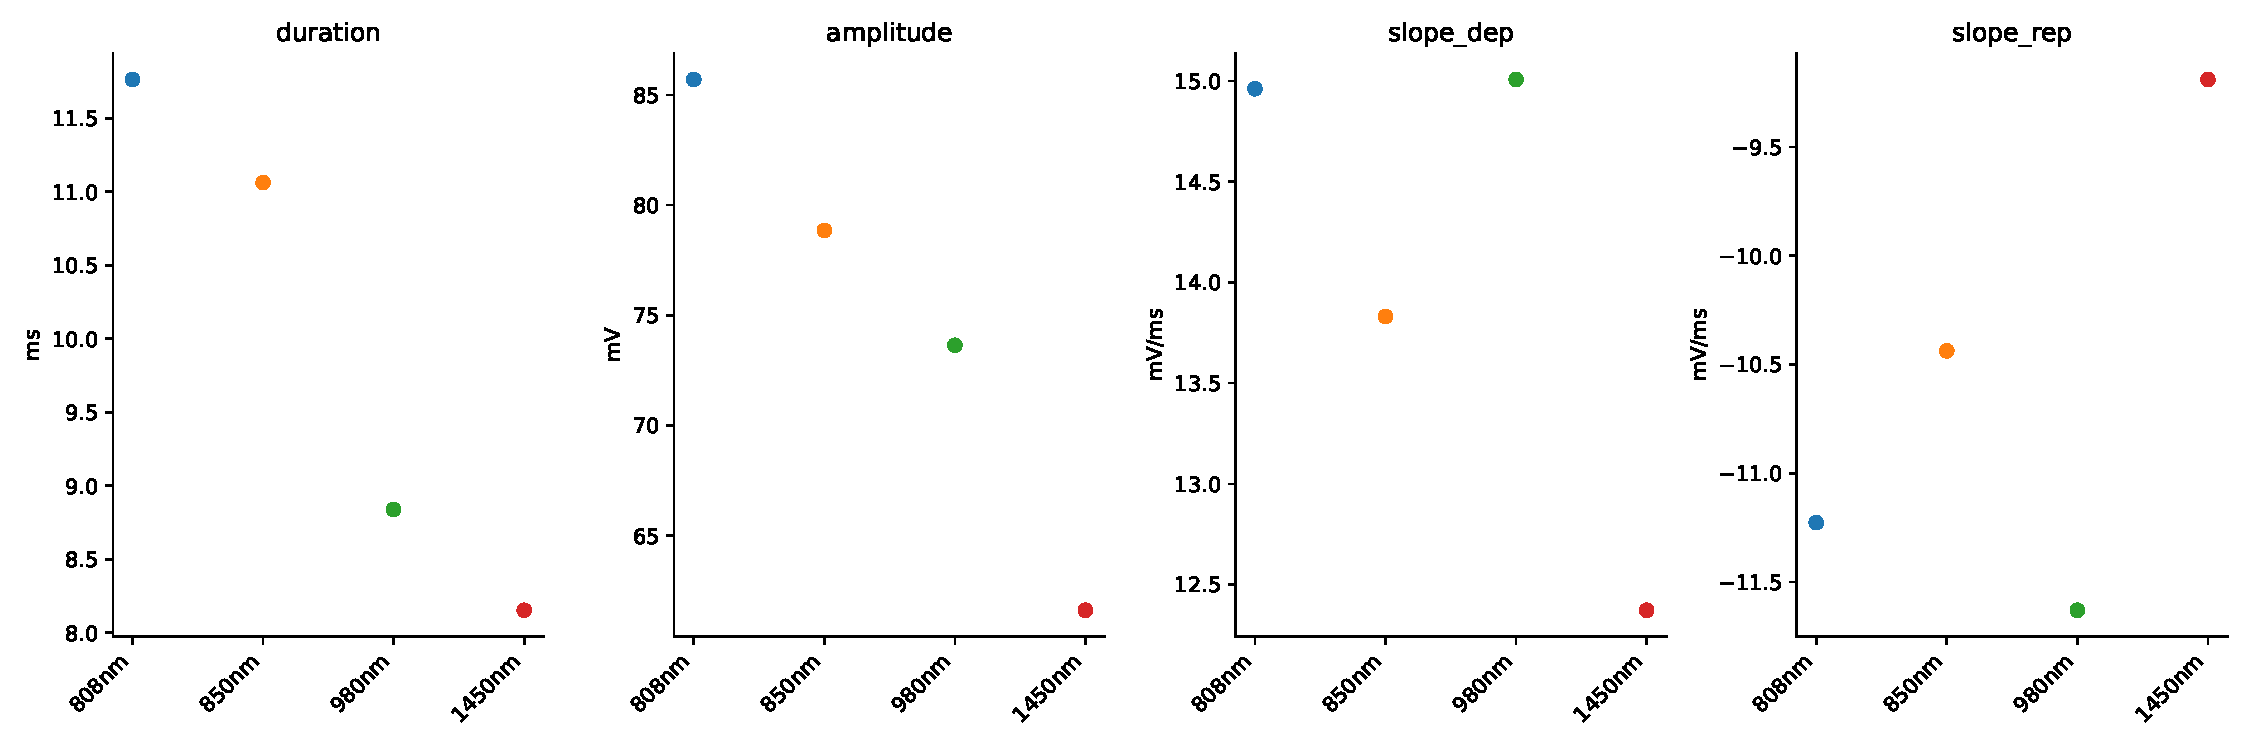
\includegraphics[width=\textwidth]{img/laser/wavelength/allmetrics.pdf}
\end{figure}
